\UseRawInputEncoding
\documentclass[a4paper, 14pt]{extarticle}

% Поля
%--------------------------------------
\usepackage{geometry}
\geometry{a4paper,tmargin=2cm,bmargin=2cm,lmargin=3cm,rmargin=1cm}
%--------------------------------------


%Russian-specific packages
%--------------------------------------
\usepackage[T2A]{fontenc}
\usepackage[utf8]{inputenc} 
\usepackage[english, main=russian]{babel}
\usepackage{cmap}
%--------------------------------------

\usepackage{textcomp}

% Красная строка
%--------------------------------------
\usepackage{indentfirst}               
%--------------------------------------             


%Graphics
%--------------------------------------
\usepackage{graphicx}
\graphicspath{ {./images/} }
\usepackage{wrapfig}
%--------------------------------------

% Полуторный интервал
%--------------------------------------
\linespread{1.3}                    
%--------------------------------------

%Выравнивание и переносы
%--------------------------------------
% Избавляемся от переполнений
\sloppy
% Запрещаем разрыв страницы после первой строки абзаца
\clubpenalty=10000
% Запрещаем разрыв страницы после последней строки абзаца
\widowpenalty=10000
%--------------------------------------

%Списки
\usepackage{enumitem}

%Подписи
\usepackage{caption} 

%Гиперссылки
\usepackage{hyperref}

\hypersetup {
	unicode=true
}

%Рисунки
%--------------------------------------
\DeclareCaptionLabelSeparator*{emdash}{~--- }
\captionsetup[figure]{labelsep=emdash,font=onehalfspacing,position=bottom}
%--------------------------------------

\usepackage{tempora}
\usepackage{amsmath}
\usepackage[dvipsnames]{xcolor}
\usepackage{listings}
\lstset{
  belowcaptionskip=1\baselineskip,
  breaklines=true,
  frame=L,
  xleftmargin=\parindent,
  language=Java,
  showstringspaces=false,
  basicstyle=\footnotesize\ttfamily,
  keywordstyle=\bfseries\color{blue},
  commentstyle=\itshape\color{purple},
  identifierstyle=\color{black},
  stringstyle=\color{red},
  numbers=left,           
  numberstyle=\tiny\color{gray}, 
  numbersep=10pt,      
  % ------------------------------
}

%--------------------------------------
%			НАЧАЛО ДОКУМЕНТА
%--------------------------------------

\begin{document}

%--------------------------------------
%			ТИТУЛЬНЫЙ ЛИСТ
%--------------------------------------
\begin{titlepage}
\thispagestyle{empty}
\newpage


%Шапка титульного листа
%--------------------------------------
\vspace*{-60pt}
\hspace{-65pt}
\begin{minipage}{0.3\textwidth}
\hspace*{-20pt}\centering

\includegraphics[width=\textwidth]{emblem}
\end{minipage}
\begin{minipage}{0.67\textwidth}\small \textbf{
\vspace*{-0.7ex}
\hspace*{-6pt}\centerline{Министерство науки и высшего образования Российской Федерации}
\vspace*{-0.7ex}
\centerline{Федеральное государственное бюджетное образовательное учреждение }
\vspace*{-0.7ex}
\centerline{высшего образования}
\vspace*{-0.7ex}
\centerline{<<Московский государственный технический университет}
\vspace*{-0.7ex}
\centerline{имени Н.Э. Баумана}
\vspace*{-0.7ex}
\centerline{(национальный исследовательский университет)>>}
\vspace*{-0.7ex}
\centerline{(МГТУ им. Н.Э. Баумана)}}
\end{minipage}
%--------------------------------------

%Полосы
%--------------------------------------
\vspace{-25pt}
\hspace{-35pt}\rule{\textwidth}{2.3pt}

\vspace*{-20.3pt}
\hspace{-35pt}\rule{\textwidth}{0.4pt}
%--------------------------------------

\vspace{1.5ex}
\hspace{-35pt} \noindent \small ФАКУЛЬТЕТ\hspace{80pt} <<Информатика и системы управления>>

\vspace*{-16pt}
\hspace{47pt}\rule{0.83\textwidth}{0.4pt}

\vspace{0.5ex}
\hspace{-35pt} \noindent \small КАФЕДРА\hspace{50pt} <<Теоретическая информатика и компьютерные технологии>>

\vspace*{-16pt}
\hspace{30pt}\rule{0.866\textwidth}{0.4pt}
  
\vspace{11em}

\begin{center}
\Large {\bf Лабораторная работа № 4} \\ 
\large {\bf по курсу <<Языки и методы программирования>>} \\ 
\large <<Реализация итераторов в языке Java>>
\end{center}\normalsize

\vspace{8em}


\begin{flushright}
  {Студент группы ИУ9-21Б Воронков А. С.\hspace*{15pt} \\
  \vspace{2ex}
  Преподаватель Посевин Д. П.\hspace*{15pt}}
\end{flushright}

\bigskip

\vfill
 

\begin{center}
\textsl{Москва 2026}
\end{center}
\end{titlepage}
%--------------------------------------
%		КОНЕЦ ТИТУЛЬНОГО ЛИСТА
%--------------------------------------

\renewcommand{\ttdefault}{pcr}

\setlength{\tabcolsep}{3pt}
\newpage
\setcounter{page}{2}

\section{Цель}\label{Sect::task}
\par 
Изучение обобщённых итераторов и экземплярных вложенных классов языка Java.  
\section{Задание}
Требуется разработать на языке Java класс с реализованным интерфейсом Comparable<T>
Класс квадратных целочисленных матриц размера n с порядком на основе 
количества элементов, нарушающих симметричность матрицы относительно 
главной диагонали. 
\pagebreak
\section{Практическая реализация}
Код файла Container.java
\begin{lstlisting}
import java.util.Iterator;
import java.util.Arrays;

public class Container<T extends Iterable<E>, E> implements Iterable<E> {
    private T[] u;
    private int size;
    public Container(T[] u) {
        this.u = Arrays.copyOf(u, u.length * 2);
        this.size = u.length;
    }
    public void add(T container) {
        if (size == u.length) {
            u = Arrays.copyOf(u, u.length * 2);
        }
        u[size++] = container;
    }
    public void remove(int index) {
        System.arraycopy(u, index + 1, u, index, size - index - 1);
        u[--size] = null;
    }
    public void set(int index, T container) {
        u[index] = container;
    }
    public Iterator<E> iterator() {return new ContainerIterator();}

    private class ContainerIterator implements Iterator<E> {
        private int pos;
        public ContainerIterator() {pos = 0;}
        private Iterator<?> now = u[pos].iterator();
        public boolean hasNext() {
            if (now == null) return false;
            return pos + 1 < size || now.hasNext();
        }
        public E next() {
            while (!now.hasNext()) {
                if (hasNext()) {
                    now = u[++pos].iterator();
                } else {
                    break;
                }

            }
            return (E)now.next();
        }
    }

}
\end{lstlisting}
\per
Код файла Test.java
\begin{lstlisting}
import java.util.Arrays;
import java.util.List;

public class Test {
    public static void main(String[] args) {
        List<Integer> a = Arrays.asList(1, 2, 3);
        List<Integer> b = Arrays.asList(4, 5);
        List<Integer> c = Arrays.asList(6, 7, 10, 8);

        List[] arr = {a, b, c};
        Container<List<Integer>, Integer> p = new Container<>(arr);

        for (Object s : p) {
            System.out.println(s);
        }
    }
}
\end{lstlisting}

\section{Результаты}
В результате лабораторной работы был создан параметризированный класс с операцией конкатенации циклов

\begin{center}
    \nopagebreak
    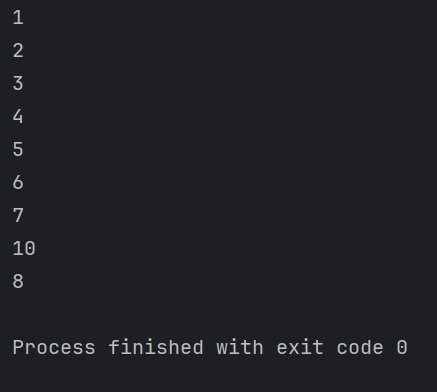
\includegraphics[width=0.85\textwidth]{lab4_1}
    \captionsetup{justification=centering}
    \captionof{figure}{Результат работы Test.java}
\end{center}

\section{Вывод}
В данной лабораторной работе были получены навыки работы с интерфейсом Iterator и Itarable
\end{document}